\mode
<article>

%% Markup
\markdownSetupSnippet{horizontalRule/singleFrame}{snippet=witiko/beamer/MU/horizontalRule/singleFrame}

%% Title page
\maketitle

\mode
<presentation>

%% Markup
\markdownSetupSnippet{horizontalRule/frameBreak}{snippet=witiko/beamer/MU/horizontalRule/frameBreak}
\markdownSetupSnippet{headingTwo/several}{snippet=witiko/beamer/MU/headingTwo/several}

%% Title page
\begin{frame}[plain]
\begin{tikzpicture}[overlay, remember picture]
  \node[anchor=south east, xshift=254.5pt, yshift=-27pt] at (current page.south east) {
    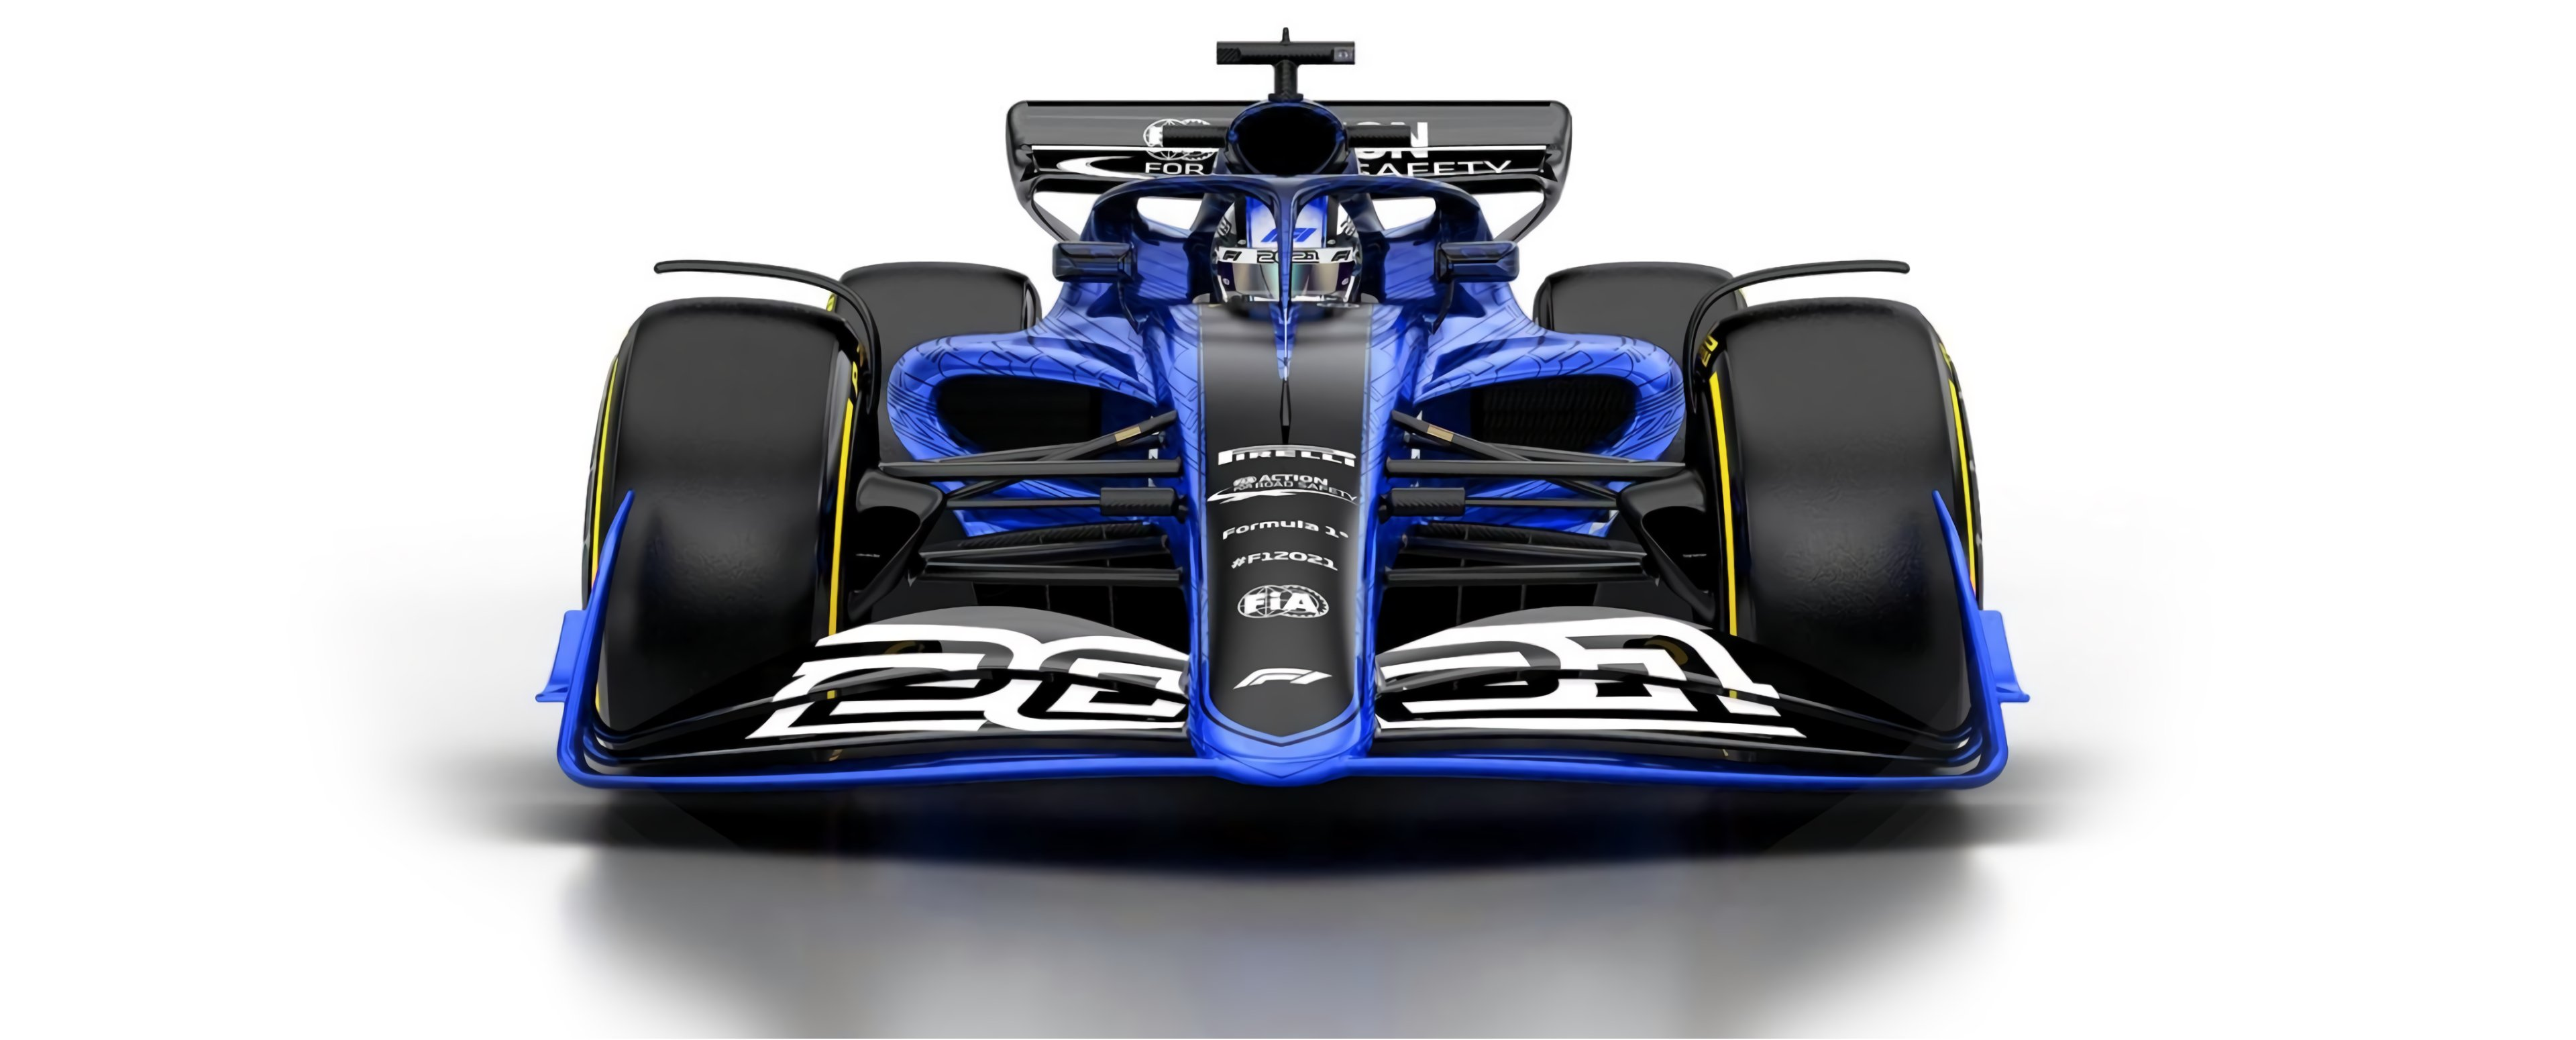
\includegraphics[height=0.91\textheight]{formula1}
  };
\end{tikzpicture}
\maketitle
\end{frame}

%% Graphics
\setkeys{Gin}{
  width = \columnwidth,
  height = \paperheight,
  keepaspectratio,
}

\mode
<article>

\part{Summary}

\markdownInput[slice=^ ^introduction]{defense.md}
\markdownInput[slice=introduction ^research-questions]{defense.md}
\markdownInput[slice=research-questions, snippet=horizontalRule/singleFrame]{defense.md}
\markdownInput[slice=thesis-structure]{defense.md}
\markdownInput[slice=digital-mathematical-libraries]{defense.md}
\markdownInput[slice=math-representations]{defense.md}
\markdownInput[slice=math-information-retrieval]{defense.md}

% ...

\part{Rebuttal}

\markdownInput[slice=oard ^oard-results-of-the-work, snippet=horizontalRule/singleFrame]{defense.md}
\markdownInput[slice=oard-results-of-the-work]{defense.md}
\markdownInput[slice=oard-thesis-structure]{defense.md}
\markdownInput[slice=oard-defense-questions]{defense.md}
\markdownInput[slice=oard-defense-questions]{defense.md}
\markdownInput[slice=skopal ^skopal-results-of-the-work, snippet=horizontalRule/singleFrame]{defense.md}
\markdownInput[slice=skopal-results-of-the-work]{defense.md}
\markdownInput[slice=skopal-thesis-structure-and-evaluation]{defense.md}
\markdownInput[slice=skopal-defense-questions]{defense.md}
\markdownInput[slice=rebuttal-conclusion]{defense.md}

\printbibliography

\mode
<presentation>

\part{Summary}
\frame{\vfill\partpage\vfill}

\section{Introduction}
\begin{frame}[fragile]
  \markdownInput[slice=introduction ^research-questions]{defense.md}
\end{frame}

\subsection{Research Questions}
\begin{frame}[fragile]{\secname}
  \markdownInput[slice=research-questions]{defense.md}
  \markdownInput[slice=thesis-structure, snippet=headingTwo/several]{defense.md}
\end{frame}

\section{Background}
\subsection{Digital Mathematical Libraries}
\begingroup
\setbeamertemplate{footline}{}
\begin{frame}[fragile, allowframebreaks=1.2]{\secname}
  \markdownInput[slice=digital-mathematical-libraries, snippet=horizontalRule/frameBreak]{defense.md}
\end{frame}
\endgroup

\subsection{Math Representations}
\begingroup
\setbeamertemplate{footline}{}
\begin{frame}[fragile]{\secname}
  \markdownInput[slice=math-representations]{defense.md}
\end{frame}
\endgroup

\subsection{Math Information Retrieval}
\begingroup
\setbeamertemplate{footline}{}
\begin{frame}[fragile, allowframebreaks=1.2]{\secname}
  \markdownInput[slice=math-information-retrieval, snippet=horizontalRule/frameBreak]{defense.md}
\end{frame}
\endgroup

\subsection{Objectives and Evaluation}
\begin{frame}[fragile]{\secname}
  \markdownInput[slice=objectives-and-evaluation]{defense.md}
\end{frame}

\section{State of the Art}
\subsection{Competitions}
\begin{frame}[fragile]{\secname}
  \markdownInput[slice=competitions]{defense.md}
\end{frame}

\subsection{Systems}
\begin{frame}[fragile, allowframebreaks]{\secname}
  \markdownInput[slice=systems, snippet=horizontalRule/frameBreak]{defense.md}
\end{frame}

\section{Accuracy}
\section{Speed}
\section{Interpretability}
\section{Conclusion}
\section{List of Author's Publications}

\begin{frame}[plain]
\vfill
\centerline{Thank You for Your Attention!}
\vfill\vfill
\end{frame}

\part{Rebuttal}
\frame{\vfill\partpage\vfill}

\section{Response to the report of prof.\ Oard}

\subsection{The Results of the Work}
\begin{frame}[fragile]{\secname}
  \markdownInput[slice=oard-results-of-the-work]{defense.md}
\end{frame}

\subsection{Thesis Structure}
\begin{frame}[fragile]{\secname}
  \markdownInput[slice=oard-thesis-structure]{defense.md}
\end{frame}

\subsection{Defense Questions}
\begin{frame}[fragile]{\secname}
  \markdownInput[slice=oard-defense-questions]{defense.md}
\end{frame}

\subsection{Text Comments}
\begin{frame}[fragile]{\secname}
  \markdownInput[slice=oard-defense-questions]{defense.md}
\end{frame}

\section{Response to the report of prof.\ Skopal}

\subsection{The Results of the Work}
\begin{frame}[fragile]{\secname}
  \markdownInput[slice=skopal-results-of-the-work]{defense.md}
\end{frame}

\subsection{Thesis Structure and Evaluation}
\begin{frame}[fragile]{\secname}
  \markdownInput[slice=skopal-thesis-structure-and-evaluation]{defense.md}
\end{frame}

\subsection{Defense Questions}
\begin{frame}[fragile]{\secname}
  \markdownInput[slice=skopal-defense-questions]{defense.md}
\end{frame}

\section{Conclusion}
\begin{frame}[fragile]
  \markdownInput[slice=rebuttal-conclusion]{defense.md}
\end{frame}

\part{\bibname}
\frame{\vfill\partpage\vfill}

\section{\bibname}
\begin{frame}[allowframebreaks]{\bibname}
\printbibliography[heading=none]
\end{frame}

\mode
<all>
